\chapter{Factoring}
\label{ch:factoring}

\chapquote{To do}{Seriously.}

When we \textit{factor} a number, we re-write it in a way that reveals its multiplicative structure. For example, we can factor 78 and rewrite it as $2\cdot39$ or as $2\cdot3\cdot13$. Indeed, you have probably been finding the \textit{prime factorization} of numbers for a while now. 

Factoring a polynomial has the same goal: to rewrite the polynomial as an equivalent multiplication problem. We will learn several important techniques for factoring, but we begin with the end in mind: an example of how factoring is helpful for solving equations.

% % % % % % % % % % % % % % % % % % % % % % % % % % % % % % % % % % % % % % % % 
\section{Quadratic equations, revisited}
\label{sec:factorsolvingpreview}

\begin{boxedexplore}[Startup exploration: Solutions and factors]
Solve the following quadratic equation using the quadrangle method that we studied in \cref{ch:quadeq}:
\[x^2 + 3x + 2 = 0\]
Then, look back at \cref{fig:tileproduct} (figure?), which shows a way of writing this quadratic trinomial as the product of two binomials.
\[(x+1)(x+2) = x^2+3x+2\]
What relationships, if any, are there between these factors and the solutions to the given equation?
\end{boxedexplore}

We solve the quadratic $x^2+3x+2=0$ using the quadrangle method, beginning with the observation that the linear term has an odd coefficient. So, we multiply through by 4: $4x^2+12x+8=0$. From here, we can draw the quadrangle diagram:

\quadrangle{2x}{3}{4x^2}{6x}{\color{red}9}

The quadrangle diagram predicts a constant term of 9, but we only have 8. So, we add 1 to both sides. Here's the full work:
\begin{commwork}
x^2+3x+2			& 0
\\
4x^2+12x+8		& 0
& multiply through by 4
\\
4x^2 + 12x + 9		& 1
& add 1 to both sides
\\
(2x+3)^2			& 1
& based on the quadrangle diagram
\\
2x+3				& 1 \OR -1
& square root of both sides
\\
2x					& -2 \OR -4
& subtract 3 throughout
\\
x					& -1 \OR -2
& divide by 2 throughout
\end{commwork}

So, we have solutions $-1$ and $-2$. Now consider the factorization $(x+1)(x+2)$. Isn't it interesting that the constants in the two factors are the opposites of the two solutions? It turns out that this connection is not a coincidence.

\subsection{Zero product property}

To explain the connection, we will turn to one of the most obvious statements in elementary mathematics. It is a statement so simple that you might be surprised that it could ever serve any truly helpful purpose.

\begin{boxeddef}[Zero product property]
If $a \cdot b = 0$, then either $a=0$ or $b=0$ (or both). In other words: if the product of two numbers is 0, then at least one of those numbers must be zero.
\end{boxeddef}

Ridiculously simple, right? But watch it in action! Consider again the original quadratic equation we were given in the startup exploration:
\[x^2 + 3x + 2 = 0.\]
We have seen that we can factor this quadratic expression into the product of two binomials. In other words, we may write:
\[(x+1)(x+2) = 0.\]
Here we have the product of two expressions, and that product equals 0. The zero product property tells us that one or the other of those factors must be equal to zero! In other words, either $(x+1) = 0$ or $(x+2)=0$.

But if $x+1=0$, then $x=-1$. So $-1$ is a solution to the equation. On the other hand, if $x+2=0$, then $x=-2$. So $-2$ is also a solution to the equation! We just found the two solutions to our quadratic without the quadrangle method!

Behold the power of factoring! When tasked with solving a quadratic equation (or any polynomial equation, really), we can sometimes attack it using factoring and the zero product property. This approach doesn't always work, and in those cases we must rely on other techniques (like the quadrangle method). But, factoring will give us an elegant way to solve equations, and teach us other things as well, for example about the graphs of polynomial functions.

In the next several sections we will progress through the levels of factoring challenge, revisit the quadrangle diagram in a rectangular format, and fill our toolbox with an impressive collection of tools and techniques.

% % % % % % % % % % % % % % % % % % % % % % % % % % % % % % % % % % % % % % % % 
\section{Factoring level 1: Greatest common factor}
\label{sec:gcf}

The greatest common factor, or GCF, of two integers is the largest number (also an integer) that divides evenly into both of the given integers. One way to find the greatest common factor of a pair of numbers is to list all of the factors of each and then hunt through both lists to find the largest number they share.

For example, suppose we wish to find the greatest common factor of 36 and 60. We list all the factors of each:
\begin{table}
\begin{tabular}{c|l}
36 & 1, 2, 3, 4, 6, 9, 12, 18, 36\\\hline
60 & 1, 2, 3, 4, 5, 6, 10, 12, 15, 20, 30, 60
\end{tabular}
\end{table}
Searching through the lists show us that 12 is the largest number they have in common, so 12 is the greatest common factor of 36 and 60. We sometimes write $\GCF(36,60)=12$.

The list-all-the-factors approach is fine for small numbers, but quickly becomes tedious if the numbers get big. For example, if we want to find the GCF of 1764 and 1890. An alternative method is to find the prime factorizations of the two numbers and compare them using a Venn diagram.

The prime factorizations of our two numbers are
\[1764=2\cdot2\cdot3\cdot3\cdot7\cdot7 \qquad\text{and}\qquad 1890=2\cdot3\cdot3\cdot3\cdot5\cdot7.\] We arrange their prime factors in a Venn diagram like the one below, placing the prime factors of each number inside the appropriate circle. If the two numbers share a factor, we place that factor (once only) in the overlapping region.

\begin{figure}
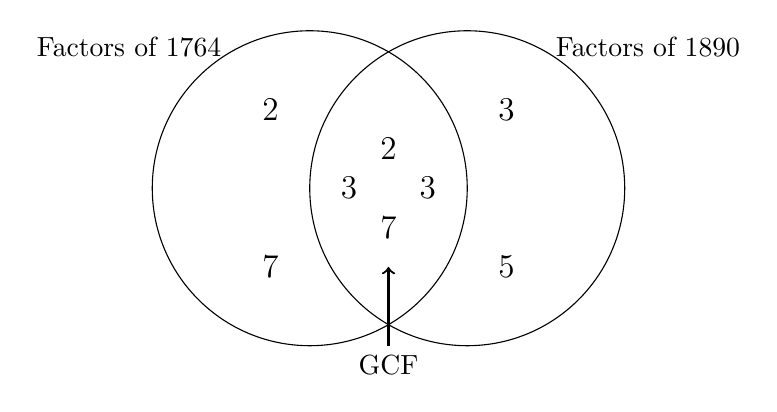
\begin{tikzpicture}
	\draw(0,0) circle[radius=2];
	\draw(2,0) circle[radius=2];
	\node at(1,0.5) {\large 2};
	\node at(0.5,0) {\large 3};
	\node at(1.5,0) {\large 3};
	\node at(1,-0.5) {\large 7};
	\node at(-0.5,1) {\large 2};
	\node at(-0.5,-1) {\large 7};
	\node at(2.5,1) {\large 3};
	\node at(2.5,-1) {\large 5};
	\node[right] at(3, 1.8) {Factors of 1890};
	\node[left] at(-1, 1.8) {Factors of 1764};
	\draw[thick, <-] (1, -1) -- (1, -2) node[below]{GCF};
\end{tikzpicture}
\end{figure}

The factors in the overlapping region are those shared by both of the numbers. The product of all the numbers in the overlap is the GCF. In this case, we have:
\[\GCF(1764, 1890) = 2\cdot3\cdot3\cdot7 = 126.\]
We will use this Venn diagram approach to tackle our first polynomial factoring challenge.

\subsection{{GCF} for polynomials}

Undoing the Distributive Property by Factoring Out the GCF

This is what we are familiar with. This is how we simplify by distributing.

 Simplify:
 3x( 2x + 5)
 3x*2x + 3x * 5
 6x2 + 15x

Now factoring takes the 6x2+ 12x (the product) and rewrites it so that you have the original, un-simplified multiplication problem. There is a lot of logic involved. You have to find the Greatest Common Factor of the terms of a polynomial. To find the GCF of a polynomial 6x2+ 15x, you have to look at each term. What do you notice about each of the terms? You should notice that both terms have x and both terms are multiples of 3. This gives you a clue to what some common factors are\ldots{} 3 and x. Now, to find the greatest common factor. You can do this systematically and prime factorize each term.

 6x2: 2 $\cdot$ 3 $\cdot$ x $\cdot$ x 
15x: 3 $\cdot$ 5 $\cdot$ x 

Circle the common factors. All of the common terms multiply together to form the GCF. What do you notice between the GCF and the previous problem? The GCF is that number that got sprinkled during the distribution. This means that if you can find the GCF, you can undo the distributive property and factor a polynomial.

Example 1

Find the GCF of 6x4 + 4x3 + 8x2 
Solution:
What do you notice about each of the terms? You may be able to find the GCF that way, or, if you can't, prime factorize each term.
6x4: 2 $\cdot$ 3 $\cdot$ x $\cdot$ x $\cdot$ x $\cdot$ x 
4X3 : 2 $\cdot$ 2 $\cdot$ x $\cdot$ x $\cdot$ x 
8x2 : 2 $\cdot$ 2 $\cdot$ 2 $\cdot$ x $\cdot$ x 

All of the terms have an x2 and all of them are even, so 2x is the GCF.
Example 2

Find the GCF of each of the following polynomials. 
1. 12x4+ 18x3
2. 32y4- 16y2
3. -4y2- 8y - 12
Solution:
1. 6x3 
2. 16y2 
3. 4 or -4 (-4 technically isn't the greatest but it is sometimes convenient to use the negative factor to change all of the signs)

Factoring out the GCF

Technically, when you undo the distributive property you are ``factoring out a monomial term.'' Now, if you can find the GCF, this is really easy. The GCF is the thing being sprinkled. The stuff left over after the GCF is taken out goes in parenthesis. It is the thing that gets the sprinkling. Now, the cool thing, is that this is so easy to check. If you want to see that you factored correctly, all you have to do is redistribute.

We will use 6x3 + 4x2 + 8x. Start by finding the GCF, which we know is 2x from example 1. The GCF is the monomial that goes outside of the ( ) in the distribution problem., whatever factors are left over from the prime factorization makes up the polynomial that goes inside of the ( ). 2x (3x2+ 2x + 4). Now, check to see if they are equivalent. Distribute the 2x or just graph both on your graphing calculator. 

If you factor out the GCFs of the polynomials in example 2, you get the following:

1. 6x3(2x + 3)
2. 16y2 (2y2 - 1)
3. 4(-y2 - 2y -3) or -4(y2 + 2y + 3)

Often, when you are asked to factor a polynomial, the first thing you should look for is a GCF that can be factored out of the problem. Actually, one of the most missed things on the assessment over factoring is forgetting to factor out a GCF. 

% % % % % % % % % % % % % % % % % % % % % % % % % % % % % % % % % % % % % % % % 
\section{Factoring level 2: Monic quadratics}

This is how to factor using algebra tiles. We are basically taking the multiplication and doing it in reverse. Instead of starting with the dimensions, we are going to start with the tiles and arrange them into a rectangle. The length and width of the rectangle will be the factors we are looking for.
How can these tiles be arranged into a rectangle?



First, you must know the polynomial being represented by the tiles. Then, experiment and turn them into a single rectangle. After that, find the length and width of the rectangle. Remember that the ``x2'' tiles have to be in the top left corner and the unit tiles have to form a rectangle in the lower right corner. The ``x'' tiles fill in the spaces.



Now all you have to do is determine what the factors are that create this rectangle. Look along the left side. It is made up of 1x and 1 unit, so the binomial is (x+1). Finally look along the top. It is made up of 1x and 2 units, so the binomial is (x+2). Therefore the factored form of x2 + 3x+2 = (x+1)(x+2). This is easy to check. Just multiply the binomials back out or use a graphing calculator.

The tiles are manipulatives that are used to show the area model of a polynomial. It is just as easy to realize that a quadratic trinomial results from the product of two binomials from experience. The multiplication of 2 binomials results in 4 terms, two of which are combined in the final step. Instead of drawing the individual tiles, you can just draw a rectangle and break it up into 4 sections. The top left section represents the quadratic term, the bottom right is the section containing the constant term. The other two sections are the two that combined to form the linear term. If you use this instead, you have to figure out how to break up the linear term. There is only one combinations that is going to work. In addition, once you figure out how to break it up and have your rectangle drawn, you find the GCF of each column to find one factor. Find the GCF of each row to find the other factor.

Quadratic Term
Part of linear term
Part of linear term
Constant Term

Of course, we want to be able to do this without the tiles and without drawing rectangles. In essence we are anti-foiling, or anti-double distributing. Think about where all of the terms in the quadratic come from in terms where/when during the process of multiplication.

1. Where does quadratic term come from?
2. Where does constant term come from?
3. Where does linear term come from?

Knowing the answers to the 3 questions above, you can factor using logic.

1. The quadratic term comes from multiplying x by x. So we know our factors have to start (x\ldots{}.)(x\ldots{})
2. Since all of the terms are positive, we know our factors have to be (x+\ldots{})(x+\ldots{})
3. We also know that the factors have to look like (x+ some number)(x + some other number)
4. So what could those numbers be? Well, we know they multiply together to give us the ``c'' term. Since the c in this case is 2, we know the two numbers have to be 1 and 2.
5. It looks like our factors are going to be (x+1) and (x+2), but we have to be sure. The way to check is to look at the ``bx'' term. We know that comes from multiplying the ``outer'' and ``inner'' terms together and adding those products together. Let's check to see if this is going to work. The ``outer'' product is 2x, the inner is 1x, the sum is 3x. That is what we were given originally, so x2+ 3x + 2 = (x+1)(x+2)

If you want to factor without the tiles, you have to ``guess and check''. Here's an organized way to do just that. It is, of course, based on the above sequence of logical steps.

1. Find the factors of the ``c'' term.
2. The factors that add up to the ``b'' term are the correct ones.
3. Check the signs to make sure they will multiply correctly!
4. Check your answer!

That is the actual procedure we are going to use to factor quadratic trinomials of the form x2 + bx + c. 
Remember to incorporate the sign of the factors of c. The final step is to always check to make sure everything works right. It is really easy to pick the wrong factors or the wrong sign on the factors. I'll go through the reasoning only on some of these, but give the solution to all of them. Remember, for this special case, I am looking for factors of c that add to b. 

Example 1

Factor: 

1. x2 + 7x + 12		2. x2 + 8x + 12		3. x2 + 2x - 3		4. x2 - 6x + 8
5. x2 + x - 12		6. x2 - 3x - 10		7. x2- 8x + 15		8. x2- 3x - 18
9. x2- 3x + 2		10. x2- 10x + 21

Solution:
1. We need to look for factors of +12 that add to 7. This means they both have to be positive. The possible factor pairs are (1, 12), (2, 6), and (3,4). Which of these pairs add up to 7? That would be 3 and 4. It seems that (x + 3)(x + 4) might be the factors. They add up to 7 and multiply out to 12. Time to check (x+3)(x+4) =x2 + 4x + 3x + 12 = x2+ 7x + 12.
2. (x + 6)(x+2)
3. We need to look for factors of -3 that add to 2. This means that one is negative and one is positive. Also that the positive one is ``bigger.'' The possible factor pairs are (1, -3) and (-1, 3). Which of these add up to +2? (-1, 3). (x - 1) (x+3) looks to be the answer. Time to check (x-1)(x+3) = x2+ 3x - x - 3 = x2+ 2x - 3
4. We need to look for factors of +8 that add to -6. This means that they both are negative. The possible factor pairs are (-1, -8), (-2, -4). Which of these add up to -6? (-2, -4). (x - 2)(x -4) might be the solution. Check: (x-2)(x-4) = x2- 4x - 2x + 8 = x2- 6x + 8
5. ( x + 4)(x - 3)
6. (x-5)(x+2)
7. (x - 3)(x-5)
8. ( x - 6)(x + 3)
9. ( x - 2)(x-1)
10. (x - 7)(x-3)

% % % % % % % % % % % % % % % % % % % % % % % % % % % % % % % % % % % % % % % % 
\section{Factoring levels 3 and 4: Two special cases}



\subsection{Level 3: Difference of squares}

\begin{boxedexplore}[Startup exploration: Factoring level 3]
The polynomials below don't look like Level 2 factoring problems, since they have only two terms. How can we change these into Level 2 problems? What happens when we factor them using Level 2 techniques?

\begin{tabularx}{\linewidth}{NNN}
x^2-9 & x^2-100 & x^2-36
\end{tabularx}
\end{boxedexplore}

We can extend each of the binomals in the startup exploration by adding a linear term with coefficient zero. Then we'd have, for example,
\[x^2+0x-9\]
To factor this, we are looking for two numbers that multiply to $-9$ and add up to 0. The natural choice is 3 and $-3$. So, we have the factorization:
\[x^2-9 = (x+3)(x-3)\]
Following this chain of reasoning, we have:
\[x^2-100 = (x+10)(x-10) \qquad\text{and}\qquad x^2-36 = (x+6)(x-6)\]

Polynomials of this form are called the \textit{difference of squares} since we have some perfect square minus a different perfect square. The resulting binomial factors are almost identical, but with different signs on their second term. They have to be of opposite sign for that $bx$ term to disappear from the final product!

\begin{boxedwarning}[Not the sum of squares!]
Important note: this is not the sum of squares! For example, we can't factor the following polynomial in the same way:
\[x^2 + 100\]
Folks can be tempted to see the sum of squares and write out a factorization, but this does not work the same way! In fact, expressions like this are never factorable in Algebra 1. (Can you explain why not?)
\end{boxedwarning}

When modeling teh difference of squares with algebra tiles, we have a picture that looks like \cref{fig:diffsquares}. The green $x$ tiles and the red $-x$ tiles zero one another out, leaving the $x^2$ tile and a collection of $-1$ tiles.

\begin{figure}
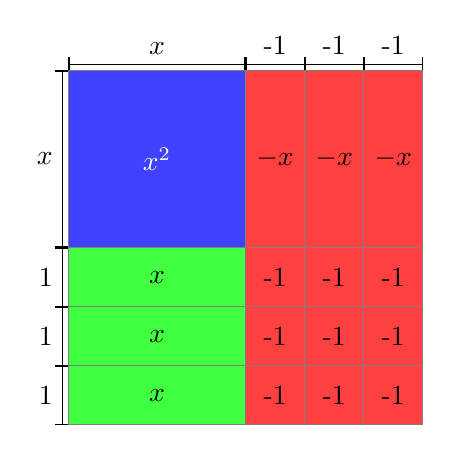
\begin{tikzpicture}[scale=0.75]
	\draw[|-|] (0,0.1) -- node[above]{$x$} (3,0.1);
	\draw[|-|] (-0.1,0) -- node[left]{$x$} (-0.1,-3);
	\draw[gray, fill=blue!75] (0,0) rectangle node[white]{$x^2$} (3,-3);
	\foreach \x in {3,...,5} {
		\draw[|-|] (\x,0.1) -- node[above]{-1} (\x+1,0.1);
		\draw[gray, fill=red!75] (\x,0) rectangle node[black]{$-x$} (\x+1,-3);
	}
	\foreach \y in {-3,...,-5} {
		\draw[|-|] (-0.1,\y) -- node[left]{1} (-0.1,\y-1);
		\draw[gray, fill=green!75] (0,\y) rectangle node[black]{$x$} (3,\y-1);
	}
	\foreach \x in {3,...,5} {
		\foreach \y in {-3,...,-5}
			\draw[gray, fill=red!75] (\x, \y) rectangle node[black]{-1} (\x+1,\y-1);
	}
\end{tikzpicture}
\caption{Difference of squares: $x^2-9=(x+3)(x-3)$}
\label{fig:diffsquares}
\end{figure}

The general form of a difference of squares, in which $a$ and $b$ can be any terms, is given below. Thinking of $a$ and $b$ as generic terms will let us expand this technique a bit further.

\begin{boxeddef}[Difference of squares]
\[a^2 - b^2= (a + b)(a - b).\]
\end{boxeddef}

\subsubsection{Beyond monics}

If the quadratic is monic, then it's leading term is a perfect square. After all $x^2 = 1x^2 = x \cdot x$. But we can have other leading terms that are also perfect squares. In fact, as we saw in \cref{ch:quadeq}, the quadratic term is a perfect square if its coefficient is a perfect square. So, for example:
\[16x^2 = 4x \cdot 4x\]
Given this idea, we can factor quadratics like:
\[16x^2 - 25 = (4x+5)(4x-5)\]
So, we have a technique now for handling non-monic quadratics, at least in certain cases.

\subsubsection{Beyond quadratics}

We are going to keep our main focus on quadratics, but it is worth mentioning that we have a technique for factoring certain higher-degree polynomials. How might we tackle this one?
\[x^4 - 16\]
In this case, $16$ if definitely a perfect square, and so is $x^4 = (x^2)^2$. So, this is the difference of squares, and we have:
\[x^4 - 16 = (x^2+4)(x^2-4)\]
We just factored a quartic polynomial, and that's something! But wait a minute -- the second factor here is again a diffrence of squares. So, we can factor even more. The simplest form is:
\[x^4 - 16 = (x^2+4)(x^2-4) = (x^2+4)(x+2)(x-2)\]
Beware at this point! Don't go ``factor crazy'' and try and factor that $x^2 + 4$. Remember: that's the sum of squares and we can't factor that (yet).

We like to call this a Goldilocks problem. Remember ``Goldilocks and the Three Bears'', the bedtime story about breaking and entering? In the story, Goldilocks goes through the bears' home messing with everything until she finds something that's ``just right''. The first bowl of porridge is too hot, the second bowl is too cold, but the third is ``just right''. The first bed is too hard, the second is too soft, but the third is ``just right''.\footnote{In the original versions of the Goldilocks story, the person who trespasses in the bears' home was an old woman -- a foul-mouthed criminal, in fact -- which, perhaps, makes a lot more sense given her actions in the story.}

We call polynomials like $x^4-16$ ``Goldilocks polynomials'' because there's a temptation to factor too little\ldots\ and a temptation to factor too much. We have to know what's ``just right''.


\subsection{Level 4: Perfect square trinomials}


\begin{boxedexplore}[Startup exploration: Factoring level 4]
Carry out the following multiplications. What patterns do you notice that relate the factors to the product?

\begin{tabularx}{\linewidth}{NNN}
(x+5)^2 & (x-4)^2 & (3x-5)x^2
\end{tabularx}
\end{boxedexplore}

A trinomial that is formed by squaring a binomial is called, naturally enough, a \gls{perfect square trinomial}. In the exponential unit (\cref{sec:exposumstopowers}), we called this raising a sum to a power. We used the quadrangle method to great benefit when solving quadratic equations (\cref{ch:quadeq}). The diagram that we drew was a kind of abstract algebra tiles picture in which all the tiles together formed a large square.

\begin{figure}
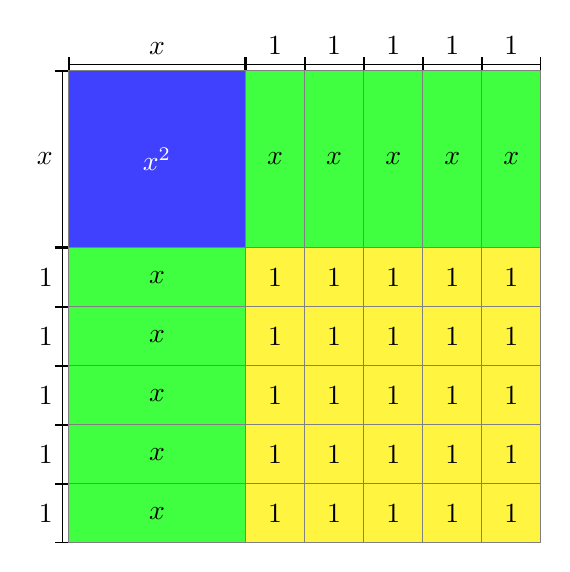
\begin{tikzpicture}[scale=0.75]
	\draw[|-|] (0,0.1) -- node[above]{$x$} (3,0.1);
	\draw[|-|] (-0.1,0) -- node[left]{$x$} (-0.1,-3);
	\draw[gray, fill=blue!75] (0,0) rectangle node[white]{$x^2$} (3,-3);
	\foreach \x in {3,...,7} {
		\draw[|-|] (\x,0.1) -- node[above]{1} (\x+1,0.1);
		\draw[gray, fill=green!75] (\x,0) rectangle node[black]{$x$} (\x+1,-3);
	}
	\foreach \y in {-3,...,-7} {
		\draw[|-|] (-0.1,\y) -- node[left]{1} (-0.1,\y-1);
		\draw[gray, fill=green!75] (0,\y) rectangle node[black]{$x$} (3,\y-1);
	}
	\foreach \x in {3,...,7} {
		\foreach \y in {-3,...,-7}
			\draw[gray, fill=yellow!75] (\x, \y) rectangle node[black]{1} (\x+1,\y-1);
	}
\end{tikzpicture}
\caption{Perfect square trinomial: $(x+5)^2=x^2+10x+25$}
\label{fig:perfsquaretri}
\end{figure}

Perfect square trinomials have some special features which make them easier to multiply and easier to factor. Notice that the first and last terms of the trinomial are both perfect squares. Note also that the $bx$ term is twice the product of the terms in the binomial that we are squaring!

\begin{boxeddef}[Perfect square trinomial]
\[(a+b)^2 = (a+b)(a+b) = a^2 + ab + ba + b^2 = a^2 + 2ab + b^2\]
\[(a-b)^2 = (a-b)(a-b) = a^2 - ab - ba + b^2 = a^2 - 2ab + b^2\]
\end{boxeddef}

As with the difference of squares, we can use this model to factor non-monic polynomials. The key is knowing when we have a perfect square trinomial and when we don't. The first, and easiest, thing to check is that the quadratic term and the constant term are both perfect squares. From there, we can imagine a candidate factorization -- but we still have to check the linear term!

\begin{boxedex}
Determing whether each of the following are perfect square trinomails. If so, write the factorization.

\begin{tabularx}{\linewidth}{NNN}
x^2-12x+36 & 9x^2+34x+25 & 64x^2 + 48x+ 9
\end{tabularx}

\exsoln\ In the first polynomial, $x^2$ is a perfect square and 36 is a perfect square. So, we might conjecture that the factorization is $(x+6)$. We have to check the linear term, which must be double the product of the terms in our binomial: $2\cdot x \cdot 6 = 12x$, which is close. To get the signs to work out, we can rely on karmic multiplication: $(-6)^2 = 36$. So, our factorization is:
\[x^2-12x+36 = (x-6)^2\]

The first and last terms of the second example should lead us to conjecture that the factorization is $(3x+5)^2$. But, if this were true then the middle term would be $2\cdot 3x \cdot 5 = 30x$. We have $34x$, and so the given trinomial is not a perfect square.

In the third example, we conjecture that the factorization is $(8x+3)^2$. This would, in turn, require the linear term to be: $2\cdot 8x \cdot 3 = 48x$. Good news, that's what we have! So, the factorization is:
\[64x^2 + 48x + 9 = (8x+3)^2\] 
\end{boxedex}

The second polynomial in the previous example \textit{is factorable}, however it is not a perfect square. More on how to tackle problems like that one in the next section!


% % % % % % % % % % % % % % % % % % % % % % % % % % % % % % % % % % % % % % % % 
\section{Factoring level 5: Factoring by grouping}

This is a general form of factoring that will allow us to factor just about anything that can be factored. To get the hang of the mechanics, we will start by factoring expressions that look a bit abstract. Then, we'll apply this technique in context.
 
\begin{boxedexplore}[Startup exploration: Factoring level 5]
Use the ``multiple distribution method'' to simplify $(a+b)(c+d)$.

Based on the patterns you notice after doing the multiplication above, rewrite the following expression as the product of two binomials.
\[pw + ps + hw + hs\]
\end{boxedexplore}

\textit{Factoring by grouping} is simply the multiple distribution method in reverse. We can multiply the two binomials in the startup exploration by first distributing the $(c+d)$ term over the other term. We would then have:
\[a (c + d) + b (c + d).\]
After distributing again, we have:
\[ac +ad + bc + bd.\]

We can visualise this using an abstract algebra tiles diagram, like so:
\quadrangleplus{a}{b}{c}{d}{ac}{ad}{bc}{bd}

How is the structure of the expression above related to this four-term expression?
\[pw + ps + hw + hs\]
Suppose we arrange the four terms in a diagram like the one above, what can we learn?
\quadrangleplus{}{}{}{}{pw}{ps}{hw}{hs}

Among these four terms, we have several pairs that share a GCF. In fact, each of the columns and rows share a GCF! If we factor out those GCFs and write them as the column headings, we have factored the expression: $(p+h)(w+s)$!
\quadrangleplus{p}{h}{w}{s}{pw}{ps}{hw}{hs}

Another way to think about what's happening is start again with the expression
\[pw + ps + hw + hs\]
and to notice that the terms $pw + ps$ have $p$ as a common factor, and the terms $hw+hs$ have $h$ as a common factor. If we factor out these GCFs, then we have:
\[p(w+s) + h(w+s)\]
This is an expression with two terms, and they share the common factor $(w+s)$. So, we can factor this out as their GCF:
\[(p+h)(w+s)\]




Note: Sometimes you will have to rearrange the factors to find the correct groups. You may also have to factor out a negative to get the leftovers to be identical.

Example 1

Factor completely.

1. ad + ac - d - c
2. 3x2 - 4x - 6x + 8
3. xy + 3y + 4x + 12
4. 3x ( x - 4) + 2( x - 4)
5. y2 ( 2x + 5) - (2x + 5)

Solution:

1. The two groups are ad + ac and -d - c . Factor out ``a'' from the first group. For the second group you will need to factor out a -1 to change the signs. Whenever you need to change the signs of an expression, you can factor out a negative 1. --> (a - 1)(d + c) 
2. The two groups are 3x2 - 4x and -6x + 8. Factor out an ``x'' from the first group. For the second group, you will need to factor out a -2, not just a two, once again to make the signs correct. -->(x -2)(3x -4)
3. The two groups are xy + 3y and 4x + 12. Factor out ``y'' from the first group. For the second group you will need to factor out a 4. --> (y + 4)(x + 3)
4. The first few steps were already done for us. --> (x - 4)(3x +2)
5. The first few steps were already done for us. --> (2x + 5) (y2 - 1)\ldots{} but this last one is tricky! First, when one of the groups has ``nothing'' in front , or only a + or -, that means that there is a ``1'' there that becomes part of the factor. Second\ldots{} my answer is ``completely factored''. You might have noticed that y2 - 1 is a difference of squares so the answer is --> (2x + 5)(y+1)(y-1) 





Now to apply these ideas to polynomials. Up until this point, we have only been able to factor ``special'' polynomials that had a certain helpful structure. Factoring by grouping is going to allow us to factor any polynomial, although we might have to do some tinkering first.

Let's use this new technique on a problem we already know how to solve. We know how to factor $x^2 + 5x + 6$ already (that's a Level 2 problem). How could we use grouping to factor this? 

First of all, we don't have enough terms: factoring by grouping requires four terms, as though we're filling in a tile diagram. So, we have to break that middle term up into 2 different terms -- we need to ``un-combine like terms''. But how?

Our options are to break $5x$ into $x + 4x$, or $2x + 3x$\ldots\ and only one of them will work. Which one? Let's try both to find out.

Option 1, we break $5x$ into $x+4x$ and try to factor by grouping.
\[x^2+5x+6 = x^2 + x + 4x + 6 = x(x +1) + 2(2x + 3)\]
When we factor the GCF from each pair of terms, the leftovers inside the parenthese are not identical. So, the resulting terms don't share a GCF and we're stuck.

Option 2, we break $5x$ into $2x+3x$ and try again.
\[x^2+5x+6 = x^2 + 2x + 3x + 6 = x(x+2) + 3(x + 2)\]
Woo hoo! The two terms here share a GCF and so, we can factor it out. In the end, we have:
\[x^2+5x+6 = (x+2)(x+3)\]
Of course, we should have known that was coming. Still, we can see how the process works.


Let's try: 2x2+ 13x + 15

If you hate grouping, you don't have to use it. You may have to spend a lot of time guessing and checking though. If I were to use pure guess and check, I have the following options: 

(x + 15)(2x + 1)		(x +3)(2x +5)		(x +5)(2x +3)		(x+1)(2x + 15)

I need to find two linear binomials so that the first term is 2x2 (formed by 2x * 1x) and the last term is 15 (formed by either 1*15 or 3*5). I then need to find the combination that will give me a 13x. This one isn't too bad because there aren't very many options. It turns out that (x+5)(2x+3) is the combination that will work. You have to be aware of the sign and check your answer!

If you want something more streamline and systematic than just guess and check, you have to factor by grouping. I just have to figure out what to break 13x into to get two groups. By inspection it is obvious that I want to break it into 3x + 10x. By grouping 2x2 + 3x + 10x + 15 = x(2x + 3) + 5(2x +3) = (x + 5)(2x +3).

Now, of course, there is a structured way to find what to break the terms up into. It's not always\ldots{} ``just look at it and figure it out''

The Procedure to factor a quadratic trinomial with grouping. (ax2 + bx + c)

1. Multiply a and c
2. Find the factors of the product ``ac'' that will add to b.
3. Split ``bx'' into two terms using the numbers found in step 2.
4. Group
5. Factor out the GCF from each group
6. Factor into binomials

Now, let's see this with an example that would be horrible to use guess and check with: 20x2 + 7x - 6

1. 20 (-6) = -120
2. Option: 1, 120; 2, 60; 3, 40; 5, 24; 	6, 20; 	8, 15; 10, 12 --> since it is negative, that means one is positive and one is negative, but they have a difference of +7 so it has to be -8 and 15. 
3. 20x2 - 8x + 15x - 6 --> (it doesn't matter which way you split the terms)
4. (20x2 - 8x) + (15x - 6) 
5. 4x (5x -2) + 3 (5x - 2) 
6. (4x + 3)(5x -2)

Example 2

Factor each of the following by grouping

1. 6x2 -7x - 5
2. 10x2 + 17x + 3
3. 8x2 + 6x - 5
4. 6x2- 19X + 10

Solution:

1. (2x +1)(3x -5)
2. (5x+1)(2x+3)
3. (2x-1)(4x+5)
4. (3x-2)(2x-5)

%\subsection{Factoring Completely}
%
%Sometimes it seems that a polynomial can't be factored. Sometimes they can't and sometimes they can. One way to check to see if a polynomial is factorable is to check the Discriminant, if it is quadratic. If the Discriminant is a perfect square, then it is likely factorable. 
%
%Another thing to check for is a GCF. Sometimes polynomials, especially special cases, are disguised by a GCF. For example, 3x2 - 75. If you notice it has 2 terms which makes it a candidate for a difference of squares, but it isn't formed by squares. The terms have a common factor, factor it out and see what you are left with. Each term has a factor of 3, so 3 (x2- 25)\ldots{} oh look, the leftovers are a difference of squares. So 3(x-5)(x+5).
%
%When you are instructed to factor completely, you have to factor until you can't factor anymore. If you leave a common factor, you will get the problem wrong. Here are the basic steps you need to remember when asked to factor.
%
%1. Factor out any GCFs
%2. Factor the resulting polynomial.
% -Check for special cases!
% 3. Check to make sure each factor is factored.
%
%
%Example 1
%
%Factor Completely: 
%1. 7x3- 343x 
%2. 4x4 - 64
%3. 2x2y - 8xy + 8y
%Solution:
%
%1. 7x(x-7)(x+7)
%2. 4(x2 + 4)(x-2)(x+2)
%3. 2y (x - 2)(x-2)

% % % % % % % % % % % % % % % % % % % % % % % % % % % % % % % % % % % % % % % % 
\section{Solving equations by factoring}

We began this chapter with an example of how factoring can be helpful when it comes to solving polynomial equations. We introduced the zero product property, which -- although is seems pretty elementary -- is a powerful tool when cleverly applied. (Have a look back at \cref{sec:factorsolvingpreview} for a refresher.)

Here's a fresh example. Suppose we want to solve the equation
\[x^2 - 3x - 40 = 0.\]
This is a Level 2 factoring problem, and so which can be factored without too much trouble:
\[(x-8)(x+5) = 0.\]
Since the product of these two equals zero, it must be that either $x-8=0$ (meaning $x=8$) or $x+5=0$ (meaning $x=-5$). So, we have found two solutions to the quadratic, and $\solset={8, -5}$. In this case, factoring might be easier than applying the quadrangle diagram approach.

Factoring works even when other approaches are possible. For example, it's easy to solve $x^2 = 25$ using the POEs. We know that $x = 5\OR-5$. But this is confirmed by a factoring approach:
\begin{commwork}
x^2 & 25
& the original equation
\\
x^2 - 25 & 0
& prepare for the zero product property
\\
(x+5)(x-5) & 0
& factor the difference of squares
\end{commwork}%
This means that either $(x+5)=0$, in which case $x=-5$, or $(x-5)=0$, in which case $x=5$. And so again, we have $\solset{5, -5}$. In this case, solving using the POEs is easier than factoring.

In some cases it's not clear which approach is easier. Suppose we have the quadratic equation
\[6x^2-7x-1=4.\]
We could carry out the quadrangle diagram procedure on this equation, as we have done many times before. Or, we could try to apply what we know about factoring. This technique is the most helpful in conjuction with the zero product property, and so we need first to have an equation equal to zero. So, we first use SPOE, which gives us  a trinomial equal to zero.
\[6x^2-7x-5=0\]
Can we factor the left-hand side? If so, it will require factoring by grouping (since neither the first nor last term is a perfect square). This means we're hunting for two numbers who product is $-30$ and whose sum is $-7$. That means $-10$ and $3$ are the numbers we're after! This gives us the factroization:
\[6x^2 - 10x +3x - 5 = 2x{\color{blue}(3x-5)} + 1{\color{blue}(3x-5)} = (2x+1)(3x-5)\]
And so this means that we have the equation:
\[(2x+1)(3x-5)=0,\]
which means that we have two equations to solve: $2x+1=0$ and $3x-5=0$. Solve these two-step equations gives us our solutions:
\[\solset{-\frac{1}{2}, \frac{3}{5}}\]
In this case, it may have been just as easy (perhaps even easier) to apply the quadrangle method.

Not every polynomial is factorable, and so not every equation can be solved by factoring. And just because an equation can't be solved by factoring doesn't mean that is has no solutions. There are quadratics that have irrational solutions that aren't factorable over integers. Conversely, if a quadratic has no solution, then it is definitely not factorable.

\addtodoitem{Should add a comment about factorable being integer coefficients...}


%Another Note: If you have a higher order equation, like a cubit, the only way you have to solve it, that isn't graphing, is factoring. 
%
%Example 1
%Problem: 
%1. (3x + 4)(x - 5) = 0
%2. 2x( 6x - 9) = 0
%3. x2 - 4x = -4
%4. x2 + 7x + 12 = 0
%5. 8x2 + 6x = 5
%6. 7x3 = 343x
%Solution:
%1. S = {-4/3 or 5}
%2. S = {0 or 3/2}
%3. S = {2}
%4. S={-3, -4}
%5. S ={ 1/2 , -5/4}
%6. S = {0,7,-7}

%Revisiting Radical Equations
%
%If you remember before spring break we did a little lesson on solving equations where the unknown was under a radical. I also said that there was one type we would have to wait to solve. Well, now is the time to solve that final type of radical equation. These equations have the unknown both under a radical and outside the radical. These types generate a quadratic equation when you square both sides, which is why we had to wait until now.
%
%Type 4: (the reason we are doing this now instead of with the radical unit)
%
%Example 2
%
%Solve: 
%
%Solution: Just like the first example, I just squared both sides of the equation, creating a quadratic after the first step.
%
%Work to find candidates for solution
%Check of candidates to find solution set
%
%Check 6
%
%
%Check -1
%
%
%Since the original equation wanted the positive root, it appears that only 6 works and -1 is an extraneous solution. S = {6}. -1 ext
%
%One simple change in the equation creates the opposite solution set. has the solution set x= {-1}, 6 ext.
%
%So be careful and check the candidates to make sure they belong in the solution set. When you solve one of the 4th type and get 2 candidates, both might work, 1 might work, or none of them will work, depending on the signs and how things play out in the solution process.

\addtodoitem{Revisit x-intercepts here}

Note for EOC\ldots{} Sometimes you will see that the EOC will ask you to find``roots'' or ``zeroes'' of a function. That means that you are trying to find x-intercepts. By now, you should have noticed that finding x-intercepts means to set the y to zero and solve the corresponding equation.

% % % % % % % % % % % % % % % % % % % % % % % % % % % % % % % % % % % % % % % % 
\subsection{Completing the square}

\addtodoitem{What do we want to say here?}

%During this lesson we are going to learn a final method for solving a quadratic equation, a method that gives us the Quadratic Formula and is the method we use to convert standard form to vertex form.
%
%Reminders about ways to Solve Quadratics:
%
%1. Graphing (finding the x-intercepts, not always exact) --> doesn't work for irrational solutions
%2. Factoring/Zero-Product Property (not everything is factorable) --> only works if you can factor
%3. Quadratic Formula --> always works, but simplifying can be annoying
%4. Completing the Square --> always works
%
%Completing the square
%
%First, we are going to do a couple of example problems to solve equations that look a specific way, kind of like vertex form. Why? Because completing the square turns all standard form quadratics equations that look like these.
%
%Example 1
%(1) 		
%(2)
%Solve each of the following with a radical. 
%(1) 
%(2) 
%
%Solution:
%Remember, when you chose to perform a root in the process of solving, you have to add ±.
%
%
%		
%Now, if you can solve all of those, then, you are ready to learn how to complete the square. The only thing you have to do is convert the quadratic to the appropriate form, a perfect square trinomial on one side a number on the other side. The first step is to convert into . It seems like voodoo, but it is based on really knowing the pattern for a PST. First, you get the coefficient of the quadratic term to be 1 by division. Then you remove the term that is preventing the quadratic from being a PST, the constant term. You add or subtract it off, then figure out what you have to add to make a PST, based on the linear term. You know that in order for the quadratic to be a PST, you have to halve the linear term and square it for the constant term. There is a very set procedure to do this.
%
%Steps to follow to complete the square.
%
%1. Move the constant using SPoE to the side opposite the variables. This should leave the linear and quadratic terms. 
%2. Divide to make sure the coefficient of the quadratic term is 1. You should have something that looks like x2 + \#x = \#
%3. Add the square of ? the coefficient of the linear term to both sides to make sure the side with the variables is a perfect square. 
%4. Factor the left side. 
%
%Let's work an example to show this process. 
%
%Example 2
%
%Solve: 
%
%1. Move the constant term
%2. no need to divide, quadratic coefficient =1
%3 \& 4. Complete the Square, divide linear coefficient by 2, square it, add it to both sides. Then factor the polynomial side.
%5. Solve
%
%Solution:
%
%
%The beauty of completing the square is that it combines factoring and opposite operations to solve and the solution is pretty much simplified by the time you find it. You just have to be really comfortable with figuring out what to add to a quadratic to turn it into a PST.
%
%Here are some more examples.
%
%Example 3
%
%Solve: 
%
%(1) 	(2) 	 (3) 
%
%
%Solution:
%
%1.
%2.
%3.

% % % % % % % % % % % % % % % % % % % % % % % % % % % % % % % % % % % % % % % % 
\subsection{Quadratic formula}

At the end of our study of quadratic equations, in \cref{sec:quadformulapreview} to be precise, we used the quadrangle method to solve a generic quadratic equation. It was an ugly bit of alphabet soup, but it is yet another way to solve a quadratic equation.

\begin{boxeddef}[The quadratic formula]
The solutions to the quadratic equation $ax^2 + bx + c=0$ (where $a\neq0$) are given by the formula:
\[x=\frac{-b\pm\sqrt{b^2-4ac}}{2a}.\]
\end{boxeddef}

\addtodoitem{What do we want to say here?}

%Since completing the square is such a rigid procedure, it is possible to do it for the general form quadratic and derive a formula for solving quadratics. See if you can follow the steps below, which is the derivation of the quadratic formula. As you follow the steps, you should see parts of the formula starting to emerge.
%
%
%I'm going to follow the same steps for completing the square. 
%
%First, subtract the constant term. 
%
%Then divide by a to make the coefficient of the quadratic term 1.
%
%Add the square of half of the coefficient of the linear term.
%
%There is some work simplifying the right side, common denominators and rearrangement into a familiar form.
%
%Then factor the polynomial side. This gives you a perfect square, so square root both sides. Don't forget the +/-.
%
%Simplify the radical remaining, remembering that you have only multiplication and division properties for radicals, and none for addition/subtraction.
%
%Finally, get that x by itself\ldots{} and there you have the quadratic formula.
%
%
%Converting from Standard to Vertex
%
%Once you've figured out how to complete the square, you can try to convert a standard from quadratic function into a vertex form. There is a reason why it is sometimes called ``completed square'' form. You have to complete the square. The y on the other side does complicate things slightly. You can't divide both sides by the coefficient of the quadratic term. You have to factor it out and be very careful about what you add to both sides to complete the square.
%
%Example 1
%
%Convert into vertex form. 
%
%Solution:
%Since the coefficient of the quadratic is 1, you don't have to worry about the division.
%
%
%Example 2
%
%Convert into vertex form. 
%
%Solution:
%Since the coefficient of the quadratic is 3, you need to factor the 3 out. When you add to complete the PST, you don't just add 1, you add 3 to both sides.

% % % % % % % % % % % % % % % % % % % % % % % % % % % % % % % % % % % % % % % % 
\subsection*{Chapter summary}

Wow! Think of how far you have come! For one thing, we have reached the apex of our work with quadratics. We have various tools for solving quadratic equations: the quadrangle method, the factoring method, and the quadratic formula. We can graph quadratic functions, and manipulate them in a variety of ways. We can manipulate radical expressions. That's quite a skill set!

Plus, we've seen a glimpse of what lies beyond quadratics. We have tinkered with other polynomials: factoring a quartic and even solving a cubic equation!

If we add this list of skills to everything that came before -- everything we learned about linear functions, systems of equations and inequalities, exponential functions -- well\ldots\ we have come quite a long way.

The only thing left to say is: Congratulations! 



\addtodoitem{A short list of things to add is found at the end of the chapter.}

To add:

irreducible

factored form -- connect back

x-intercepts -- connect back

completing the square -- connect back

solve a cubic
